\chapter{Numerical Results in the Time-Driven Approach}
This chapter is dedicated to presenting the results obtained by applying the Stochastic Reachability approach (discussed in Chapter \ref{chpt:Model_Description}) to asset allocation. We recall that the output of the ODAA algorithm (see Theorem (\ref{thm:rec_algo})) is a sequence of allocation maps $\pi^{\star}=\{\mu_0^{\star},\ldots,\mu_{N-1}^{\star}\}$. For any portfolio realization $x \in \mathbb{R}$ at time $k \in \mathbb{N}$, the maps $\mu_k^{\star}$ provides us with the optimal asset allocation $\mu_k^{\star}(x)=\bm{u}_k^{\star}$; for instance, if $\bm{u}_k^{\star}= \begin{bmatrix}
0.2 & 0.2 & 0.6
\end{bmatrix}^T$ this means that 20\% of investor's wealth should be allocated to the first asset class, 20\% to the second one and the remaining 60\% to the third one. Objective of this chapter is to see what form these maps have at different time instant. The chapter unfolds as follows: in Section \ref{sec:The_Dataset} the dataset is presented and summarized by some sample statistics, in Section \ref{sec:Allocation_Maps} the parameters of the asset allocation problems are set and the allocation maps for the different models discussed in Chapter \ref{chpt:assetclass_returns} are reported.

\section{The Dataset}\label{sec:The_Dataset}
Our asset class menu consists of cash, bond and equity. To represent these markets we adopt the indexes presented in Table \ref{tab:indexes}.
\begin{table}[h] \label{tab:indexes}
	\centering
	\begin{tabular}{@{}lll@{}} \toprule
		Label & Asset Class & Index\\ \midrule
		C & Money Market & iShares Short Treasury Bond ETF\\
		\addlinespace[0.5em]
		B & US Bond  & Northern US Treasury Index \\
		\addlinespace[0.5em]
	    E &	US Equity &  {S\&P 500}\\ \bottomrule
		\addlinespace[0.5em]
	\end{tabular}
	\caption{Asset class and relative index}
\end{table}
The dataset is composed of daily time series from 23 January 2010 to 15 April 2016. Data is downloaded from Yahoo Finance which is also where the reader is referred for more details of index composition. Asset class returns and their risk profile are summarized in Figure \ref{fig:assetclassReturns} and Table \ref{tab:sampleStatistics}.
\begin{figure}[h]\label{fig:assetclassReturns}
	\centering
	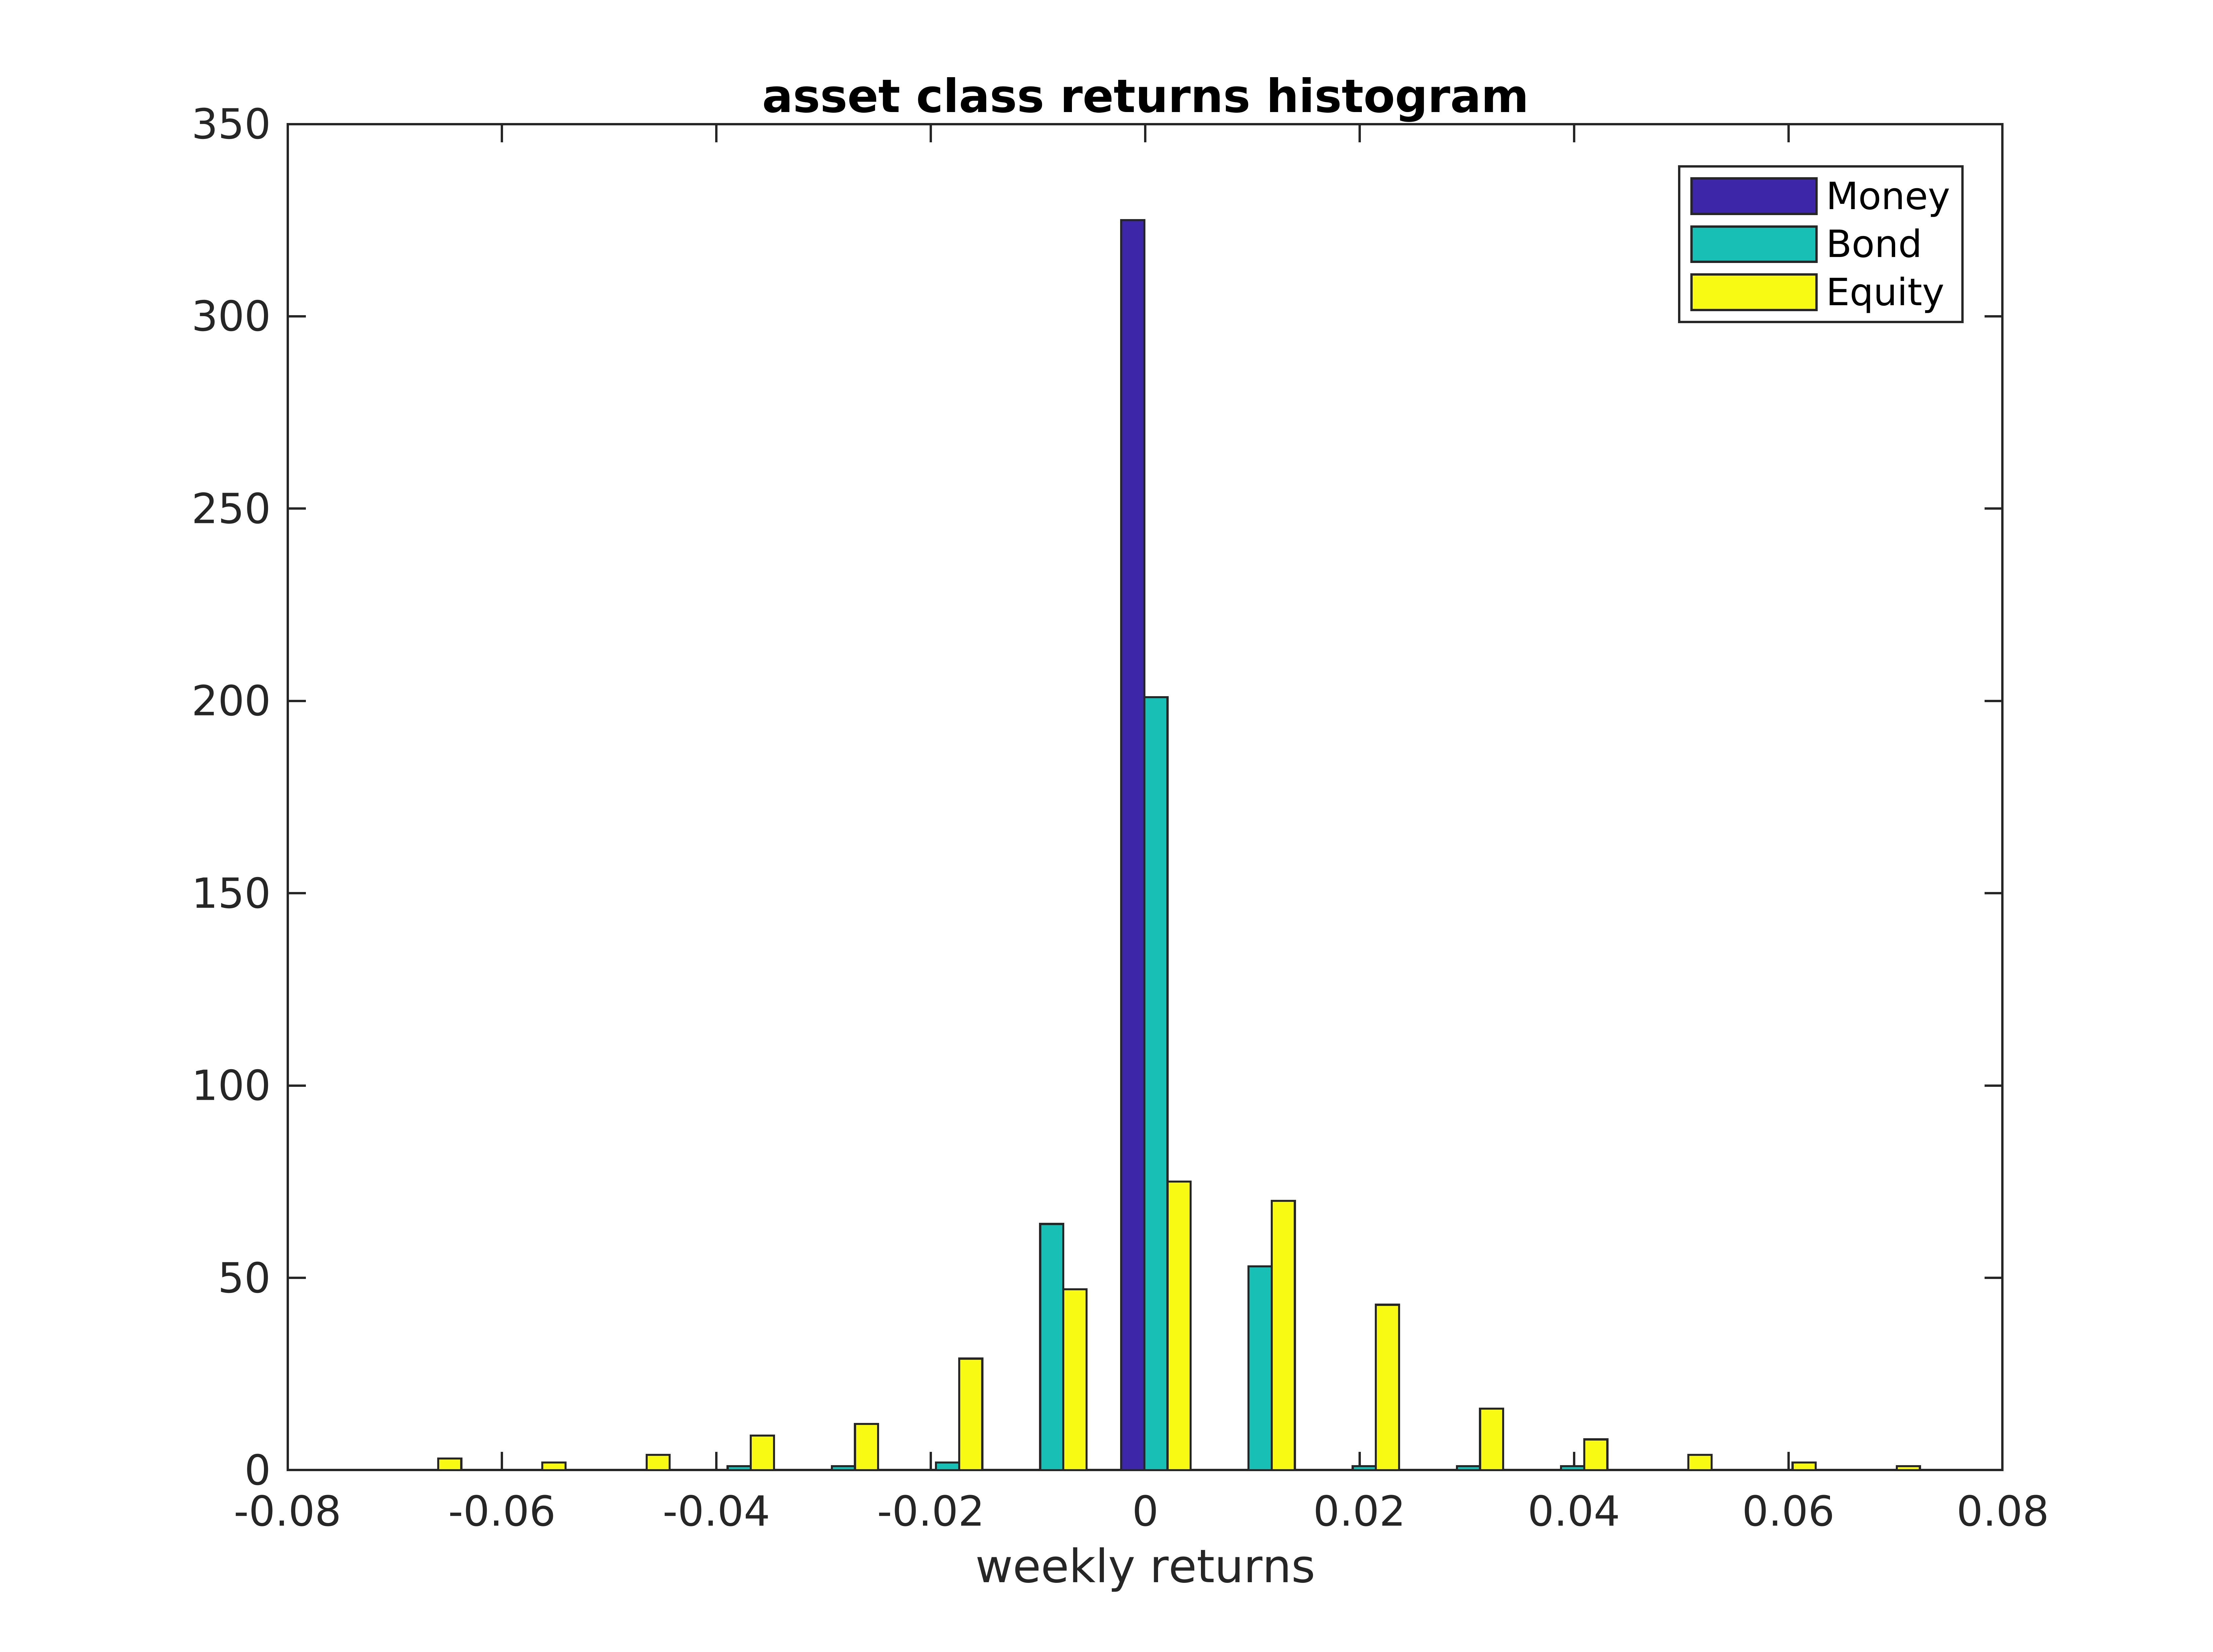
\includegraphics[scale=0.6]{Images/ReturnsHist.png}
	\caption{Weekly asset class returns histogram.}
\end{figure}
\begin{table}[H]\label{tab:sampleStatistics}
	\centering
	\begin{tabular}{@{}llll@{}} \toprule
		Statistic & C & B & E \\ \midrule
		Mean Return (ann) & 0.064\%  & 3.40\% & 11.44\%\\
		\addlinespace[0.5em]
		Volatility (ann) & 0.113\%  & 4.81\% & 14.81\% \\
		\addlinespace[0.5em]
		Median (ann) &	0\% & 4.48\% & 16.35\% \\
		\addlinespace[0.5em]
		Skewnwss & 0.262 & -0.0621 & -0.36 \\
		\addlinespace[0.5em]
		Kurtosis & 3.90 & 10.62 & 4.42 \\
		\addlinespace[0.5em]
		Monthly $V@R_{0.95}$ & 0.0807\% & 3.68\% & 14.18\%\\
		\addlinespace[0.5em]
		Max Drawdown & 0.106\% & 5.87\% & 23.98\% \\
		\addlinespace[0.5em]
		Mean Drawdown & 0.020\% & 1.5\% & 4.62\% \\
		\addlinespace[0.5em]
		Sharpe ratio & 0 & 0.692 & 0.767 \\ \bottomrule
		\addlinespace[0.5em]
	\end{tabular}
	\caption{Asset class returns sample statistics}
\end{table}
Moreover, the sample correlation matrix is  
\[ 
\begin{bmatrix}
1 & 0.166 & -0.075 \\
  &  1    & -0.454 \\
  &       &  1
\end{bmatrix}
\]
and the asset class returns do not come from a Gaussian distribution (p-value of the Henze-Zirkler multivariate normality test is zero).
\section{Allocation Maps}\label{sec:Allocation_Maps}

\begin{figure}[h]
	\centering
	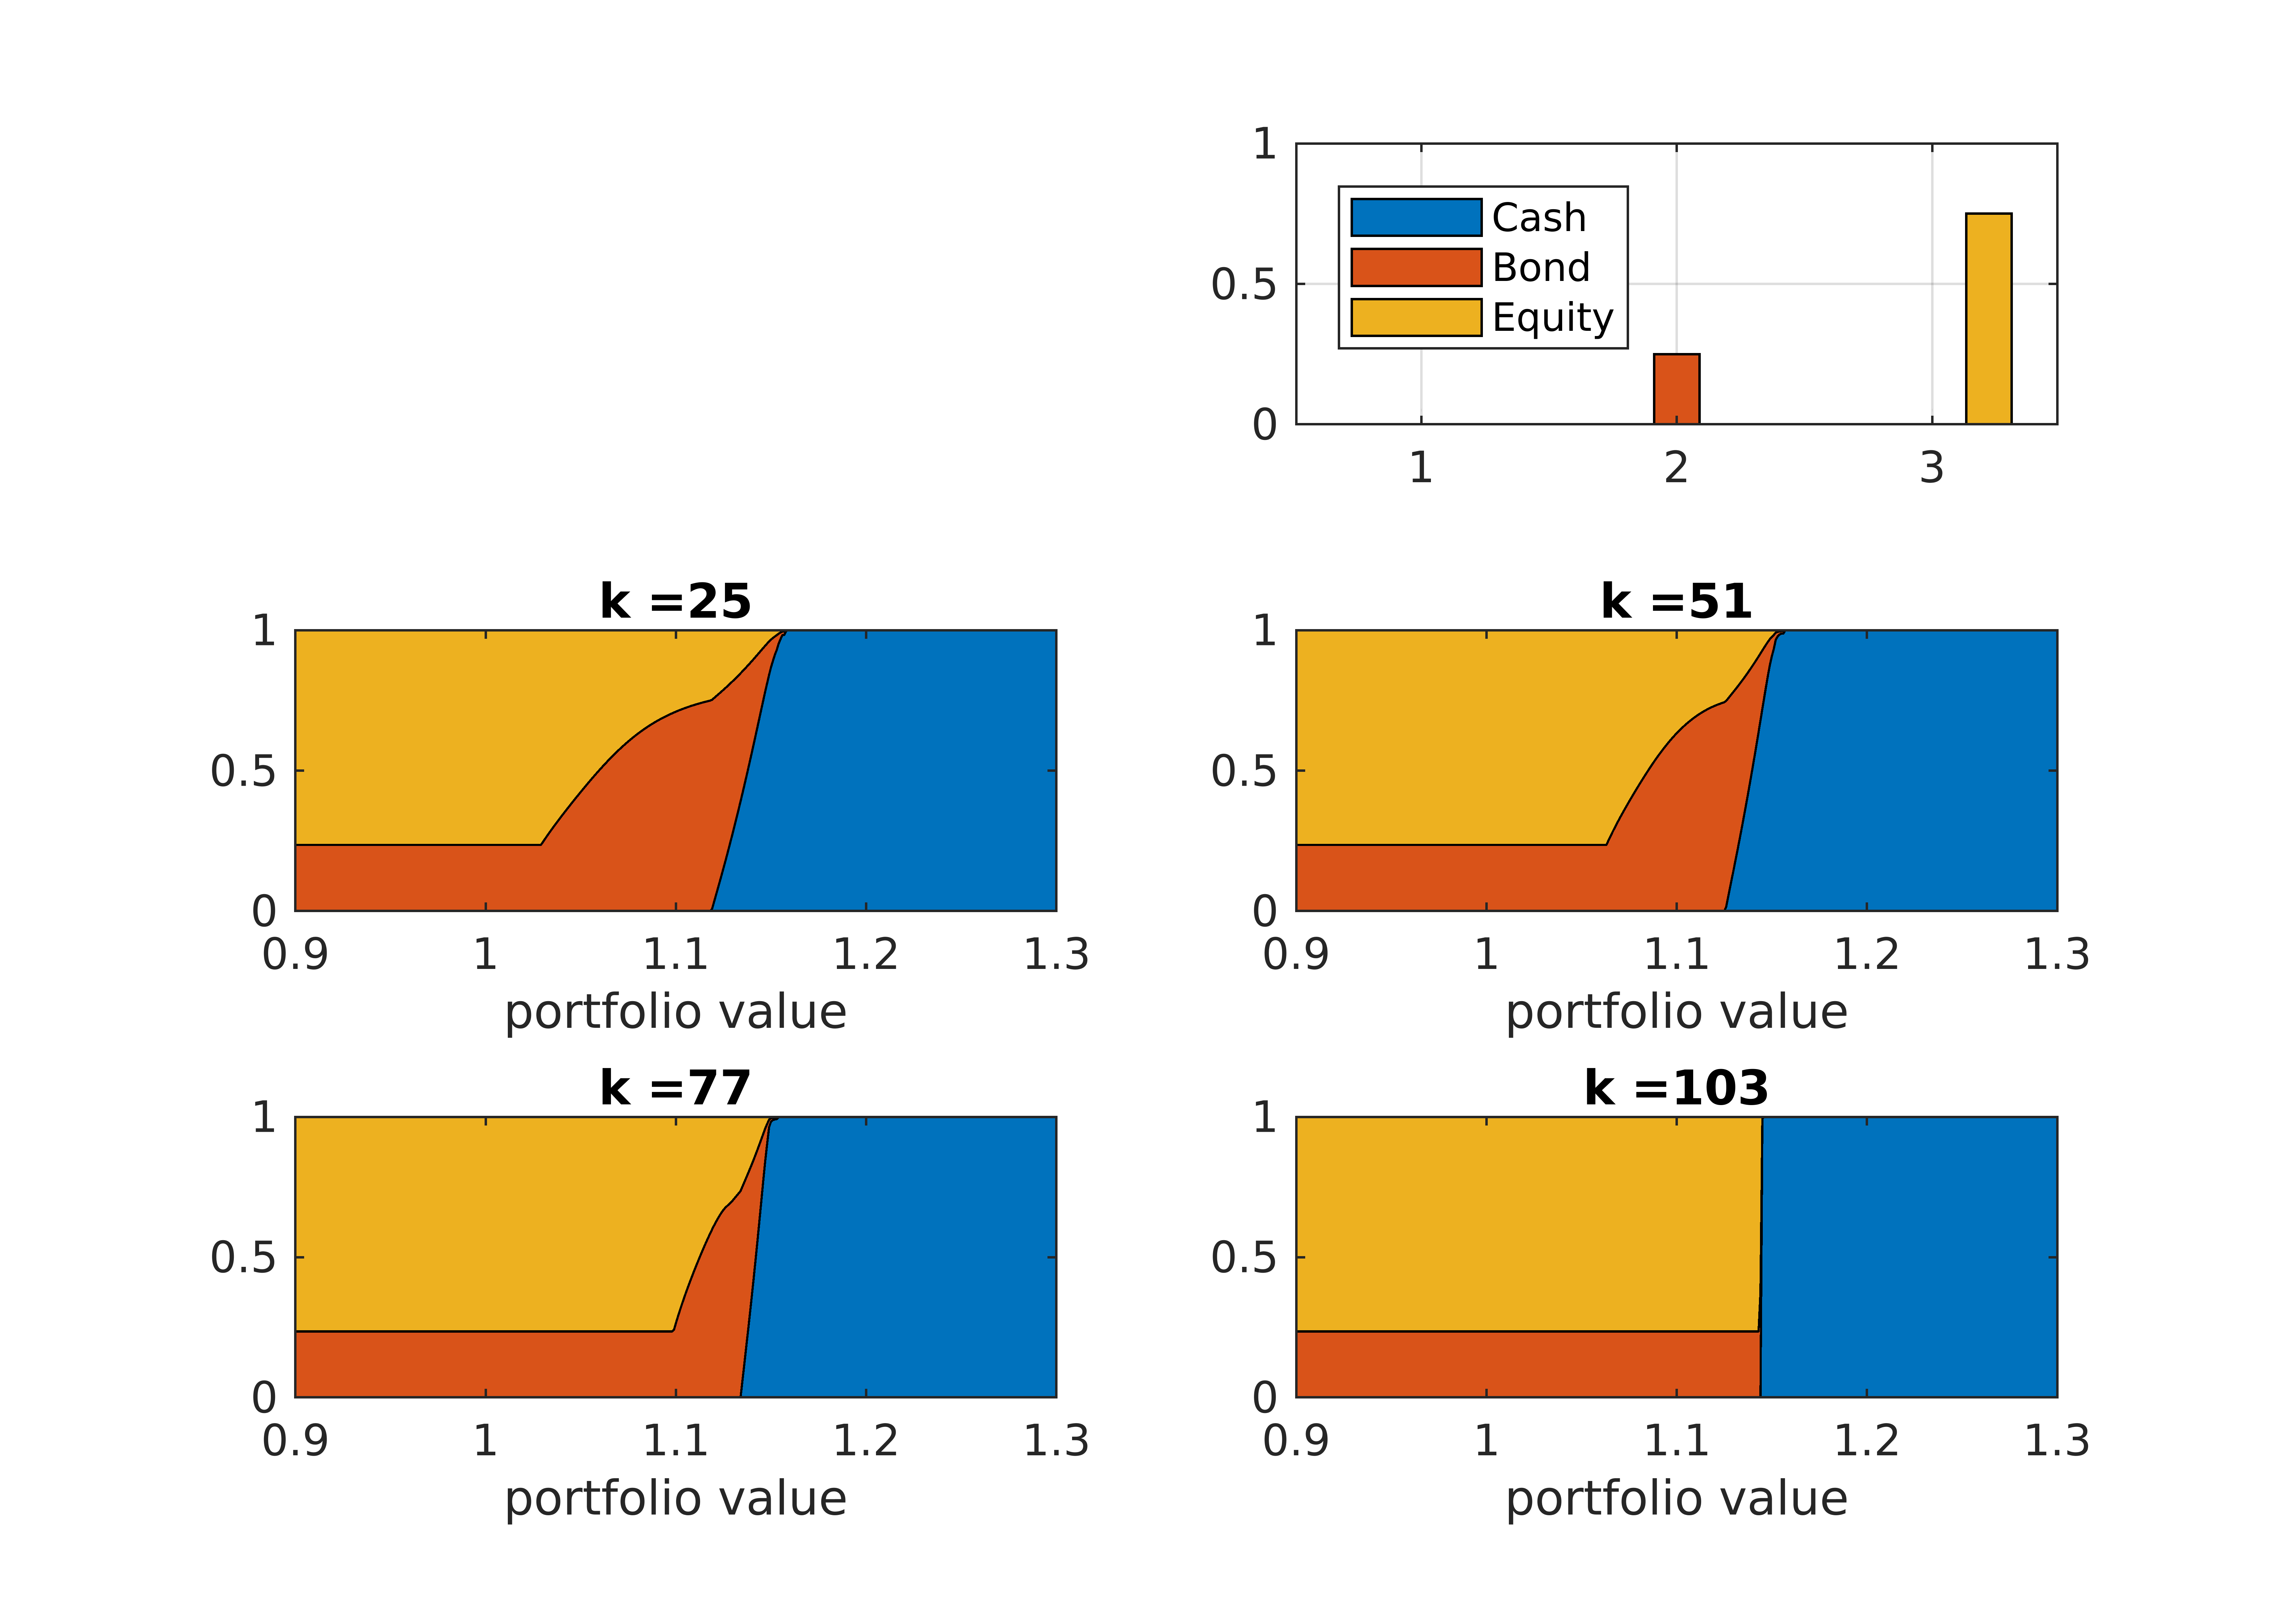
\includegraphics[scale = 0.9]{Images/mapsMixturewk.png}
	\caption{Weekly asset class returns histogram.}
\end{figure}


\begin{table}[]
	%\renewcommand{\arraystretch}{2}
	\centering
	\begin{tabular}{@{}*{10}{c}@{}}
		\toprule
		& \multicolumn{3}{c}{G} & \multicolumn{3}{c}{GM} & \multicolumn{3}{c}{NIG} \\
		\addlinespace[0.5em]
		\cmidrule(l){2-4} \cmidrule(l){5-7} \cmidrule(l){8-10} 
		& wk & m & q 	& wk & m & q 	& wk & m & q\\
		\addlinespace[0.5em]
	$p^{\star}$ & 3\% & 3\% & 3\% & 78.90\%  & 58.09\% & 5\% & 8\% & 8\% &9\%  \\
	\addlinespace[0.5em]
	$p_{MC}$ & 3\% & 3\% & 3\% & 78.92\%  & 58.16\% & 5\% & 8\% & 8\% &9\%  \\
	\addlinespace[0.5em]	
	time & 3\% & 3\% & 3\% & 2\%  & 3\% & 5\% & 8\% & 8\% &9\%  \\	\bottomrule
	\end{tabular}
\end{table}

\begin{table}[]
	
	\centering
	\begin{tabular}{@{}*{4}{c}@{}}
		\toprule
	Moment	& G & GM & NIG \\
		\addlinespace[0.5em]
		\midrule	
	$\mu_{x_{k+1}}$	& & & \\
	\addlinespace[0.5em]	
	$\sigma_{x_{k+1}}$	& & & \\
	\addlinespace[0.5em]
	$\gamma_{x_{k+1}}$	& & & \\
	\addlinespace[0.5em]
	$\kappa_{x_{k+1}}$	& & & \\
	\addlinespace[0.5em]
	\bottomrule
	\end{tabular}
\end{table}
